\documentclass[conference,a4paper]{IEEEtran}
% IEEE conference layout. Replace the class/options only if a venue supplies
% a different official template. Do not alter margins to force a page count.
\usepackage[T1]{fontenc}
\usepackage[utf8]{inputenc}
\usepackage{cite}
\usepackage{amsmath,amssymb}
\usepackage{graphicx}
\usepackage{booktabs,tabularx,array}
\usepackage{xcolor}
\usepackage{tikz}
\usetikzlibrary{arrows.meta,positioning,fit,backgrounds,shapes.geometric,calc}
\usepackage{url}
\usepackage{balance}
\usepackage[hidelinks]{hyperref}
\urlstyle{same}
\newcolumntype{Y}{>{\raggedright\arraybackslash}X}
\definecolor{ink}{HTML}{18334D}
\definecolor{bluewash}{HTML}{EAF2F8}
\definecolor{teal}{HTML}{147D83}
\definecolor{tealwash}{HTML}{E8F5F3}
\definecolor{amber}{HTML}{A46B13}
\definecolor{amberwash}{HTML}{FFF4DB}
\definecolor{slate}{HTML}{536579}
\tikzset{
  block/.style={draw=ink!65,fill=bluewash,rounded corners=2pt,
    align=center,font=\sffamily\footnotesize,inner sep=6pt,line width=.65pt},
  gate/.style={block,draw=amber,fill=amberwash},
  data/.style={block,draw=teal,fill=tealwash},
  flow/.style={-{Latex[length=2mm]},line width=.8pt,draw=ink},
  softflow/.style={flow,dashed,draw=slate},
  tag/.style={font=\sffamily\scriptsize\bfseries,text=ink,align=left},
  edge label/.style={font=\sffamily\scriptsize,fill=white,inner sep=2pt}
}
\hyphenation{Forge-Web front-end back-end work-space}
\begin{document}

\title{ForgeWeb: Architecture-First\\Full-Stack Web Application Generation}
\author{
\IEEEauthorblockN{Pratyush Manas\IEEEauthorrefmark{1}, Rajeev Kumar\IEEEauthorrefmark{2},
Sachin Yash Raj\IEEEauthorrefmark{3}, Sanaa Kumari\IEEEauthorrefmark{4}}
\IEEEauthorblockA{Department of Computer Science and Engineering\\
BMS Institute of Technology and Management, Bengaluru, India\\
\IEEEauthorrefmark{1}1BY23CS163\quad
\IEEEauthorrefmark{2}1BY23CS171\quad
\IEEEauthorrefmark{3}1BY23CS192\quad
\IEEEauthorrefmark{4}1BY23CS202}
}
\maketitle

\begin{abstract}
Generating a useful web application from a short description requires more than producing source code. The interface must reflect the requested product, frontend and backend files must share a consistent contract, and users need a way to review decisions before implementation begins. This paper presents ForgeWeb, an architecture-first prototype that organizes these activities into an inspectable workflow. The system converts a natural-language prompt into structured requirements and an architecture document, requests explicit user approval, and then generates React frontend and Python FastAPI backend artifacts. Configurable language-model providers support planning and implementation, while domain-aware local fallbacks preserve the workflow when a provider is unavailable. A project workspace exposes source files, isolated HTML previews, version snapshots, export, and a graph linking requirements to implementation artifacts. We describe the implemented architecture, the approval boundary, provider routing, and the distinction between structural checks and execution-based validation. A reproducible local evaluation passes all fourteen existing workflow and HTTP tests and the platform type checks. These results support the feasibility of the orchestration and workspace design; they do not establish production readiness or universal correctness of generated applications. The work provides a practical foundation for evaluating prompt fidelity, full-stack integration, and evidence-based acceptance in AI-assisted web development.
\end{abstract}

\begin{IEEEkeywords}
AI-assisted software engineering, full-stack generation, architecture approval, large language models, requirement traceability, web application prototyping.
\end{IEEEkeywords}

\section{Introduction}
Large language models have made natural-language code generation a practical component of software development. Codex and the HumanEval evaluation introduced a widely used way to measure whether generated functions satisfy executable tests~\cite{chen2021codex}. APPS extended evaluation to programming problems described in natural language~\cite{hendrycks2021apps}, while AlphaCode demonstrated the importance of sampling and behavioral filtering for more demanding programming tasks~\cite{li2022alphacode}. These advances motivate systems that can help a user move from a product idea to an application.

Web application generation introduces requirements that are not captured by a single function. A restaurant booking site needs a menu, reservation inputs, and availability feedback; a store needs product discovery, a cart, and an order workflow. Both may use the same frontend framework, but their information architecture, interactions, and visual identity should differ. A successful generator must also coordinate frontend requests with backend routes, preserve the user's decisions, and make failures visible.

ForgeWeb addresses this problem through an architecture-first workflow. The user submits a product description, inspects a proposed specification and \texttt{ARCHITECTURE.md}, and chooses whether to edit or approve it. Code generation begins after that approval. Generated files remain visible in a project workspace together with a preview, validation records, and version history. The objective is to make the transition from intent to implementation easier to inspect and revise.

The contribution is a systems prototype and an implementation study, not a new foundation model. Specifically, this paper describes: (i) an explicit approval boundary between planning and generation; (ii) a common specification used by frontend and backend generation; (iii) provider routing with a visible local fallback; and (iv) a workspace that associates requirements, source files, checks, and versions. The evaluation reports reproducible local checks and identifies where stronger execution and user studies are still needed.

\section{Problem Definition and Objectives}
Users often express a software requirement as a short, incomplete description. The description may mix functional needs, preferred colors, branding, security expectations, and examples. If generation starts immediately, the system can commit to an unsuitable layout or data model before the user has inspected those assumptions. Repeated templates can make unrelated products appear similar, and a visually convincing preview can hide missing backend behavior. Provider failures further complicate the process when replacement output is mistaken for a successful model response.

The problem is therefore to transform a prompt into a reviewable set of frontend and backend artifacts while preserving product intent and exposing the limits of available evidence. Let $p$ denote a prompt, $S$ the proposed specification, $a$ the approval decision, and $F$ the generated file set. ForgeWeb follows
\begin{equation}
p \xrightarrow{\mathrm{plan}} S,
\qquad (S,a) \xrightarrow{a=\mathrm{approved}} F.
\label{eq:approval}
\end{equation}
Equation~\eqref{eq:approval} describes an ordering constraint rather than a claim that approval guarantees correctness. Approval confirms the user's intended scope; validation must separately examine implementation evidence.

The objectives are to create an architecture file before generating source, allow the user to correct the plan, preserve explicit design instructions, and produce frontend and Python backend artifacts from the approved specification. Additional objectives are to expose readable source, support previews and reversible versions, retain provider provenance, and associate requirements with generated files. Production hosting, strong tenant isolation, and universal end-to-end correctness are outside the demonstrated prototype boundary.

\section{Literature Review}
\subsection{Code Synthesis and Evaluation}
CodeGen studies program synthesis using multiple turns that decompose a task into smaller specifications~\cite{nijkamp2022codegen}. InCoder supports infilling and editing with context on both sides of the generated region~\cite{fried2023incoder}. These approaches motivate structured generation and later revision, although neither is itself a complete user-facing application builder.

CodeT uses generated tests to help select candidate programs~\cite{chen2022codet}. EvalPlus shows that inadequate test suites can accept incorrect programs and change the apparent ranking of models~\cite{liu2023evalplus}. LiveCodeBench broadens evaluation across generation, execution, and repair while addressing contamination concerns~\cite{jain2024livecodebench}. BigCodeBench emphasizes complex instructions and combinations of library calls~\cite{zhuo2024bigcodebench}. Together, these studies support a central design decision: a file being present, or a preview rendering, must not be treated as proof of complete functional correctness.

\subsection{Software Engineering Agents}
SWE-bench evaluates changes to real repositories using issue descriptions and executable checks~\cite{jimenez2024swebench}. SWE-agent examines how an agent's interface to repository tools affects its software engineering performance~\cite{yang2024sweagent}. These settings are closer to application maintenance than isolated code completion, but differ from generating a new product from a customer brief.

ChatDev organizes development through communicating specialist agents~\cite{qian2024chatdev}, and MetaGPT encodes standardized workflows into multi-agent coordination~\cite{hong2023metagpt}. AutoGen provides a flexible framework for conversations involving agents, tools, and humans~\cite{wu2023autogen}. Conversely, Agentless demonstrates the value of a simpler localization, repair, and validation pipeline~\cite{xia2024agentless}. ForgeWeb adopts explicit role and artifact boundaries, but its current implementation uses coordinated task records and server functions. This should not be confused with evidence that independent autonomous agents have been deployed for every role.

\subsection{Planning, Feedback, and Context}
ReAct combines reasoning with actions that obtain environmental feedback~\cite{yao2023react}. Reflexion retains verbal feedback between attempts~\cite{shinn2023reflexion}, while Self-Refine iteratively revises output using self-generated feedback~\cite{madaan2023selfrefine}. Chain-of-thought and Plan-and-Solve prompting study intermediate reasoning and task decomposition~\cite{wei2022cot,wang2023plansolve}. ForgeWeb's architecture document serves a related organizational purpose, but is an explicit product artifact reviewed by the user rather than a claim to reproduce these prompting methods.

Retrieval-augmented generation connects generation to external information~\cite{lewis2020rag}. RepoCoder applies iterative retrieval and generation to repository-level completion~\cite{zhang2023repocoder}. These approaches are relevant to future edits spanning many files. The current ForgeWeb prototype passes a structured specification to generation; it does not implement a repository retrieval index.

\subsection{Visual Fidelity and Security}
Design2Code evaluates frontend generation from website screenshots and highlights challenges in reproducing visual elements and layout~\cite{si2025design2code}. Its relevance to ForgeWeb is the need for visual evaluation beyond source-code validity. Prompt-specific colors and page structure require their own checks, alongside functional tests.

Pearce \emph{et al.} study security weaknesses in generated code~\cite{pearce2022security}. Perry \emph{et al.} examine how AI assistance can affect both code security and users' confidence~\cite{perry2023security}. These findings motivate separating generated security artifacts from verified security behavior. An access-control file is useful evidence of intended structure, but it does not establish that every protected operation enforces the correct policy.

\begin{table}[t]
\caption{Research Themes and Their Role in ForgeWeb}
\label{tab:related}
\centering\footnotesize
\begin{tabularx}{\columnwidth}{@{}p{.25\columnwidth}YY@{}}
\toprule
Theme & Research emphasis & Design implication \\
\midrule
Code synthesis & Programs from natural language & Generate modular artifacts from explicit scope. \\
Evaluation & Tests, execution, complex tasks & Distinguish structural evidence from behavior. \\
Software agents & Roles, tools, repair workflows & Make task scope and acceptance visible. \\
Planning/context & Decomposition, feedback, retrieval & Preserve an approved specification for later stages. \\
UI and security & Visual fidelity and unsafe output & Evaluate appearance and security separately. \\
\bottomrule
\end{tabularx}
\end{table}

The research gap considered here is practical integration: a small web-generation prototype needs an understandable approval step, explicit frontend/backend artifacts, prompt-sensitive presentation, failure provenance, and inspectable project history in one workflow. Table~\ref{tab:related} summarizes the design rationale. It is not a benchmark ranking of the cited systems.

\section{System Architecture}
\subsection{User Layer}
The user layer is a React and TypeScript application. A central composer accepts the prompt, a proposal view presents requirements and architecture, and a workspace exposes files, preview, database information, and versions. The navigation drawer provides access to saved projects and a new conversation. ForgeWeb's own visual theme is separate from the style requested for a generated application.

The preview uses a sandboxed iframe with script and form permissions. It renders a stored HTML artifact and supports different viewport sizes. The iframe is a browser isolation measure; it is not a containerized environment for running arbitrary backend code. A preview may demonstrate interactions with local data even when the generated Python service has not been started.

\begin{figure*}[t]
\centering
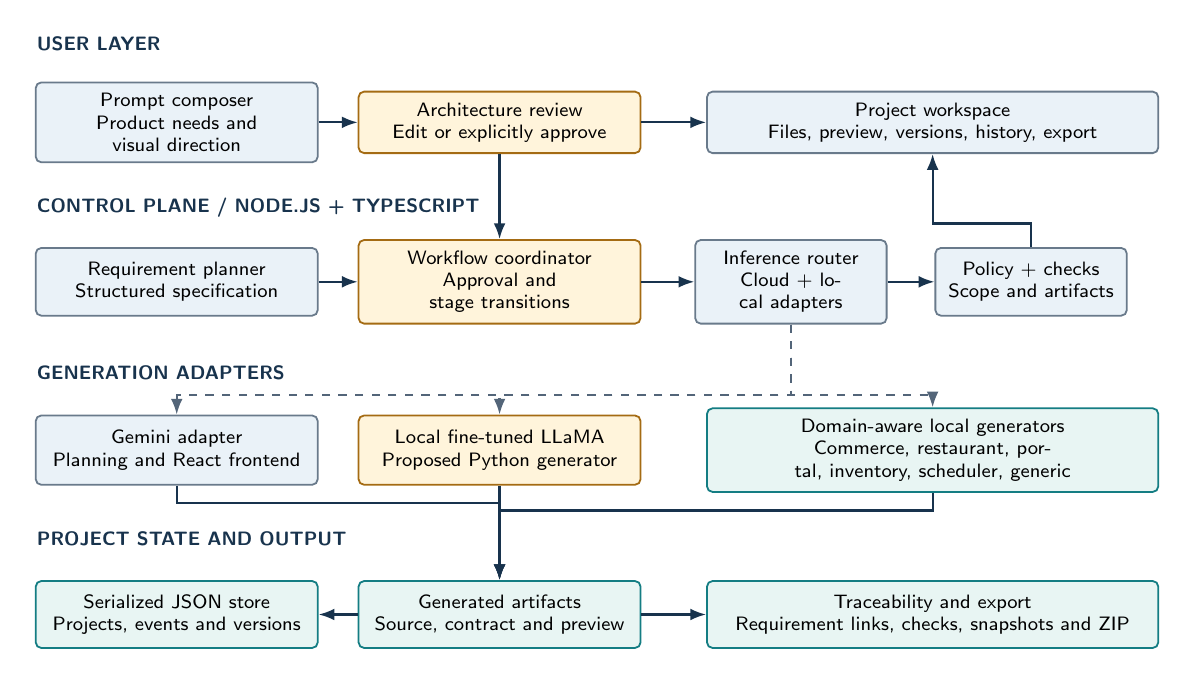
\begin{tikzpicture}[x=1cm,y=1.25cm,block/.append style={font=\sffamily\scriptsize,inner sep=4pt}]
\node[tag,anchor=west] at (0,0.45) {USER LAYER};
\node[block,text width=3.3cm,minimum height=.78cm] (prompt) at (1.9,-.35) {Prompt composer\\\scriptsize Product needs and visual direction};
\node[gate,text width=3.3cm,minimum height=.78cm] (approval) at (6,-.35) {Architecture review\\\scriptsize Edit or explicitly approve};
\node[block,text width=5.45cm,minimum height=.78cm] (workspace) at (11.5,-.35) {Project workspace\\\scriptsize Files, preview, versions, history, export};
\draw[flow] (prompt)--(approval);
\draw[flow] (approval)--(workspace);
\node[tag,anchor=west] at (0,-1.22) {CONTROL PLANE / NODE.JS + TYPESCRIPT};
\node[block,text width=3.3cm,minimum height=.86cm] (planner) at (1.9,-1.97) {Requirement planner\\\scriptsize Structured specification};
\node[gate,text width=3.3cm,minimum height=.86cm] (workflow) at (6,-1.97) {Workflow coordinator\\\scriptsize Approval and stage transitions};
\node[block,text width=2.15cm,minimum height=.86cm] (router) at (9.7,-1.97) {Inference router\\\scriptsize Cloud + local adapters};
\node[block,text width=2.15cm,minimum height=.86cm] (checks) at (12.75,-1.97) {Policy + checks\\\scriptsize Scope and artifacts};
\draw[flow] (approval.south)--(workflow.north);
\draw[flow] (planner)--(workflow);
\draw[flow] (workflow)--(router);
\draw[flow] (router)--(checks);
\draw[flow] (checks.north)--++(0,.24)-|(workspace.south);
\node[tag,anchor=west] at (0,-2.89) {GENERATION ADAPTERS};
\node[block,text width=3.3cm,minimum height=.88cm] (gemini) at (1.9,-3.68) {Gemini adapter\\\scriptsize Planning and React frontend};
\node[gate,text width=3.3cm,minimum height=.88cm] (llama) at (6,-3.68) {Local fine-tuned LLaMA\\\scriptsize Proposed Python generator};
\node[data,text width=5.45cm,minimum height=.88cm] (local) at (11.5,-3.68) {Domain-aware local generators\\\scriptsize Commerce, restaurant, portal, inventory, scheduler, generic};
\draw[softflow] (router.south)--(9.7,-3.12)-|(gemini.north);
\draw[softflow] (router.south)--(9.7,-3.12)-|(llama.north);
\draw[softflow] (router.south)--(9.7,-3.12)-|(local.north);
\node[tag,anchor=west] at (0,-4.58) {PROJECT STATE AND OUTPUT};
\node[data,text width=3.3cm,minimum height=.85cm] (store) at (1.9,-5.35) {Serialized JSON store\\\scriptsize Projects, events and versions};
\node[data,text width=3.3cm,minimum height=.85cm] (artifacts) at (6,-5.35) {Generated artifacts\\\scriptsize Source, contract and preview};
\node[data,text width=5.45cm,minimum height=.85cm] (graph) at (11.5,-5.35) {Traceability and export\\\scriptsize Requirement links, checks, snapshots and ZIP};
\draw[flow] (gemini.south)--++(0,-.18)-|(artifacts.north);
\draw[flow] (llama.south)--(artifacts.north);
\draw[flow] (local.south)--++(0,-.18)-|(artifacts.north);
\draw[flow] (artifacts)--(store);
\draw[flow] (artifacts)--(graph);
\end{tikzpicture}

\caption{Implemented ForgeWeb architecture. The user layer communicates with a Node.js control plane. Provider calls occur on the server. Source files, preview HTML, graph records, and versions are stored as project artifacts. The exported customer application has its own runtime. Dashed arrows indicate optional provider paths.}
\label{fig:architecture}
\end{figure*}

\subsection{Control Plane and Persistence}
The control plane is a native Node.js HTTP service written in TypeScript. During development, Vite middleware forwards local API requests to the same request handler used by the standalone server. The workflow maintains states including planning, awaiting confirmation, generating, reviewing, validating, completed, and failed.

The implemented store serializes project data to a local JSON file. A write queue orders mutations, and persistence writes a temporary file before renaming it. Stored records include specifications, builds, tasks, events, files, graphs, and versions. This is suitable for the local prototype, but does not provide the deployment properties of a multi-instance transactional database. Earlier project architecture documents propose PostgreSQL, queues, and isolated workers; those services are future extensions rather than dependencies of the evaluated implementation.

\subsection{Provider and Generation Layer}
Generation providers implement planning and generation interfaces. In the configured split pipeline, Gemini is preferred for planning and frontend generation, while Groq is preferred for backend generation and OpenRouter can provide a fallback. Provider selection is configurable, so this routing is a deployment choice rather than a measured ranking of model quality.

The planner returns structured fields including product name, roles, entities, requirements, pages, modules, routes, data rules, and visual direction. The application validates and normalizes this response before constructing the proposal. After approval, frontend and backend manifests are combined with support files and a shared API contract. Credentials are consumed by server-side adapters and should not be included in exported projects.

When external generation fails, the workflow can use local generators specialized for commerce, restaurants, inventory, scheduling, portals, and generic sites. This mode provides predictable artifacts for supported cases. It has a smaller design space than unconstrained model generation and cannot promise an entirely unique design for every prompt. The recorded generator mode and fallback message are therefore part of the result, not incidental diagnostic details.

\subsection{Project Workspace and Traceability}
The workspace stores each file's path, content, digest, and requirement identifiers. A version snapshot captures the generated file set so that users can inspect, export, edit, or restore it. Export validation checks the selected snapshot before creating a ZIP archive. The database tab describes the generated application's intended entities; it does not mean that a production database has already been provisioned.

Figure~\ref{fig:architecture} separates the platform from its output. Figure~\ref{fig:structure} shows the generated project structure and the runtime boundary between a preview and an independently launched application.

\section{Methodology}
\subsection{Prompt Interpretation and Architecture}
The workflow first validates the prompt and extracts product intent. Explicit naming and visual instructions are preserved during normalization. For example, a request for a light-cream client portal should influence the portal's style rather than inherit ForgeWeb's dark interface. Product classification guides the local fallback while the provider plan can supply more detailed pages, components, and domain rules.

The specification combines functional requirements, assumptions, architecture, and provider provenance. It records an architecture document that the user can read before any implementation is accepted. Editing returns the user to the prompt for revision. Approval records the intended specification and permits the workflow to continue, as shown in Fig.~\ref{fig:flow}.

\begin{figure}[t]
\centering
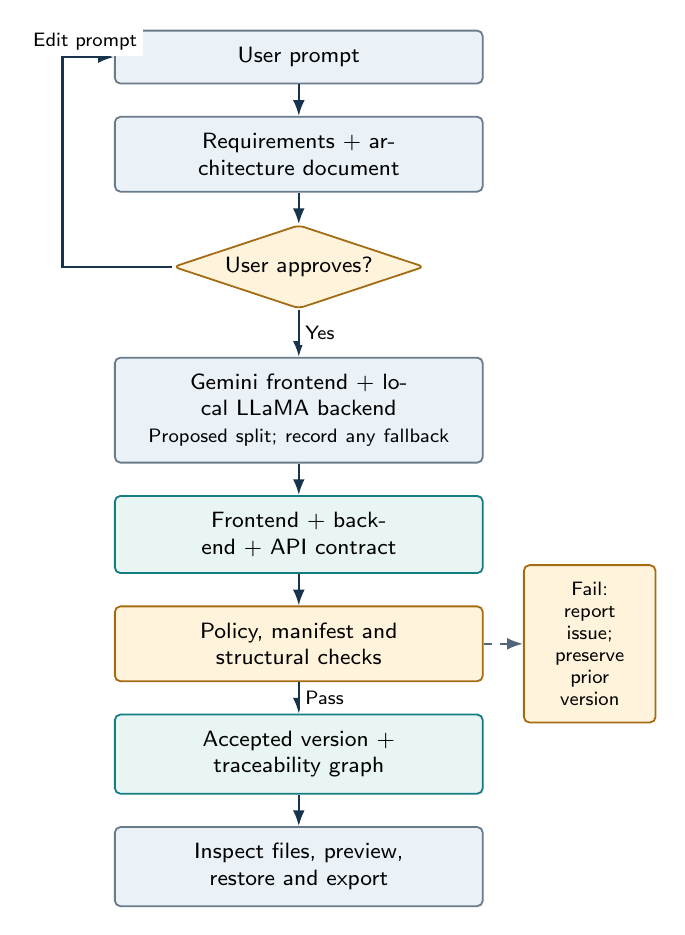
\begin{tikzpicture}[node distance=4mm]
\node[block,text width=4.25cm] (prompt) {User prompt};
\node[block,text width=4.25cm,below=of prompt] (plan) {Requirements + architecture document};
\node[gate,diamond,aspect=3,inner sep=2pt,below=of plan] (gate) {User approves?};
\node[block,text width=4.25cm,below=6mm of gate] (gen) {Gemini frontend + local LLaMA backend\\\scriptsize Proposed split; record any fallback};
\node[data,text width=4.25cm,below=of gen] (files) {Frontend + backend + API contract};
\node[gate,text width=4.25cm,below=of files] (check) {Policy, manifest and structural checks};
\node[data,text width=4.25cm,below=of check] (save) {Accepted version + traceability graph};
\node[block,text width=4.25cm,below=of save] (preview) {Inspect files, preview, restore and export};
\draw[flow] (prompt)--(plan);
\draw[flow] (plan)--(gate);
\draw[flow] (gate)--node[edge label,right]{Yes}(gen);
\draw[flow] (gate.west)--(-3,0 |- gate.west) |- node[edge label,pos=.72,above]{Edit prompt} (prompt.west);
\draw[flow] (gen)--(files);
\draw[flow] (files)--(check);
\draw[flow] (check)--node[edge label,right]{Pass}(save);
\draw[flow] (save)--(preview);
\node[gate,text width=1.25cm,font=\sffamily\scriptsize,right=5mm of check] (fail) {Fail:\\report issue;\\preserve prior version};
\draw[softflow] (check.east)--(fail.west);
\end{tikzpicture}

\caption{Prompt-to-project data flow. The user can revise the proposal before confirmation. Generation proceeds through model routing or a recorded local fallback, then through policy and structural checks. Failed checks prevent acceptance of the candidate.}
\label{fig:flow}
\end{figure}

\subsection{Contract-Guided Artifact Generation}
The approved specification is the common input to generation. The intended output includes React source, CSS, a Python FastAPI entry point, Pydantic schemas, access-control source, test artifacts, and documentation. A shared JSON contract describes the routes and domain data that should connect the frontend and backend.

Contract generation reduces avoidable ambiguity, but consistency still requires testing. Two files referring to the same contract can implement different behavior. For example, a reservation form and endpoint may disagree on a date format or required identifier. Such mismatches require requests against the running generated service and assertions on the response, beyond checking that both files exist.

\begin{figure}[t]
\centering
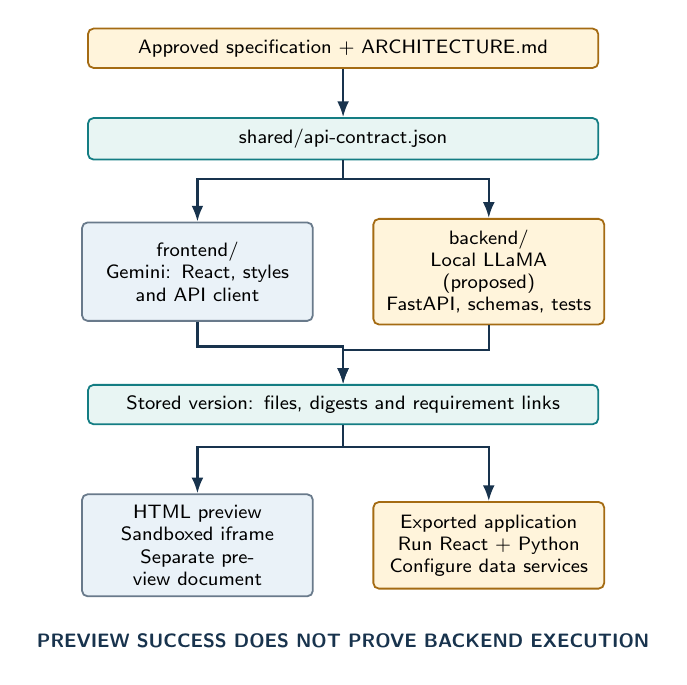
\begin{tikzpicture}[x=1cm,y=1.25cm,block/.append style={font=\sffamily\scriptsize,inner sep=4pt}]
\node[gate,text width=6.2cm] (spec) at (0,0) {Approved specification + ARCHITECTURE.md};
\node[data,text width=6.2cm] (contract) at (0,-.92) {shared/api-contract.json};
\node[block,text width=2.65cm,minimum height=1.25cm] (front) at (-1.85,-2.27) {frontend/\\\scriptsize Gemini: React, styles\\and API client};
\node[gate,text width=2.65cm,minimum height=1.25cm] (back) at (1.85,-2.27) {backend/\\\scriptsize Local LLaMA (proposed)\\FastAPI, schemas, tests};
\draw[flow] (spec)--(contract);
\draw[flow] (contract.south)--++(0,-.19)-|(front.north);
\draw[flow] (contract.south)--++(0,-.19)-|(back.north);
\node[data,text width=6.2cm] (version) at (0,-3.62) {Stored version: files, digests and requirement links};
\draw[flow] (front.south)--++(0,-.25)-|(version.north);
\draw[flow] (back.south)--++(0,-.25)-|(version.north);
\node[block,text width=2.65cm,minimum height=1.1cm] (prev) at (-1.85,-5.05) {HTML preview\\\scriptsize Sandboxed iframe\\Separate preview document};
\node[gate,text width=2.65cm,minimum height=1.1cm] (run) at (1.85,-5.05) {Exported application\\\scriptsize Run React + Python\\Configure data services};
\draw[flow] (version.south)--++(0,-.22)-|(prev.north);
\draw[flow] (version.south)--++(0,-.22)-|(run.north);
\node[tag,align=center] at (0,-6.02) {PREVIEW SUCCESS DOES NOT PROVE BACKEND EXECUTION};
\end{tikzpicture}

\caption{Structure of a generated project and its runtime boundary. The shared contract guides both source sets. The stored HTML preview is separate from the React application and Python service that a developer runs after export. Database infrastructure must be configured for that application.}
\label{fig:structure}
\end{figure}

\subsection{Engineering Roles and Scope Control}
ForgeWeb creates records for planning, implementation, review, and validation. Each record carries its objective, requirement identifiers, path scope, acceptance criteria, and policy provenance. The policy reflects four principles: clarify material assumptions, prefer a small sufficient solution, keep changes within scope, and require observable evidence.

The implementation references the project's Karpathy-derived policy material and gstack-inspired workflow notes as engineering resources. These repositories are not counted among the twenty-five research papers. In the current code, review checks requirement coverage and file budgets, and validation checks expected artifacts and other structural conditions. The roles are useful orchestration boundaries, but the review function is not an independent model performing a semantic audit.

\subsection{Validation and Graph Construction}
Let $R$ be the approved requirements and $F$ the accepted files. Each file $f$ stores a set of requirement identifiers $T(f)$. An artifact coverage indicator can be written as
\begin{equation}
C_{\mathrm{artifact}}=
\frac{|\{r\in R:\exists f\in F,\;r\in T(f)\}|}{|R|}.
\label{eq:coverage}
\end{equation}
This measure detects missing links. It does not measure how well the implementation satisfies a requirement; all requirements could be attached to one inadequate file. Behavioral coverage must be measured independently using requirement-specific assertions.

The current graph contains project, requirement, task, file, and validation nodes. Edges associate project membership, assigned tasks, files, and checks. File digests allow the workspace to identify stored content. Although some edge names express satisfaction, they represent recorded mappings rather than formal proof. The external Code Review Graph engine is identified as an integration target; the evaluated workflow constructs its own artifact graph and does not demonstrate an upstream parser-based call graph.

The acceptance boundary may be expressed as
\begin{equation}
\mathrm{Accept}(F)=A\land P(F)\land M(F)\land V_s(F),
\end{equation}
where $A$ denotes approval, $P$ path and scope checks, $M$ manifest and mapping checks, and $V_s$ the implemented structural checks. Stronger deployment acceptance should additionally require $V_b$, execution-based behavior and integration checks. Keeping $V_s$ and $V_b$ distinct prevents a structural validation badge from being interpreted as a complete security or functionality guarantee.

\section{Implementation and Reproducibility}
The inspected implementation uses React, TypeScript, Vite, and a Node.js control plane. FastAPI is the target of generated Python backend artifacts rather than the framework running the ForgeWeb control API. The source directories separate the user interface, workflow, provider adapters, policy, project storage, and domain-specific generation logic.

Reproduction begins by installing the repository dependencies, providing server-side provider configuration when live generation is required, and running the development command. The platform's test command uses the Node test runner. Test fixtures create temporary stores and use deterministic generation or an injected provider implementation; they do not require live provider credentials. Type checking covers both the platform frontend and server.

The paper package includes an evidence note mapping claims to source files and recorded command results. Provider/model settings can change independently of the platform. Consequently, a future live-generation study must record exact model identifiers, prompt text, provider responses, retry conditions, and artifact digests. A passing fixture-based run cannot be reused as evidence of a later provider's output quality.

\section{Experimental Setup, Results, and Analysis}
\subsection{Evaluation Questions}
The local evaluation asks whether the workflow enforces approval before source generation, whether supported prompt categories produce their expected artifact structures, and whether workspace operations preserve recoverable project state. It also checks the configuration path through a provider test double and verifies rejection of invalid prompts and out-of-scope files. These questions concern implementation behavior, not comparative model intelligence.

The existing suite was rerun for this manuscript. All fourteen top-level tests passed, with no failed or skipped tests. The TypeScript checking command also completed successfully. Table~\ref{tab:results} groups the tests by the behavior under observation. Some tests contain multiple assertions; the total is the number of top-level test cases, not the number of assertions or generated applications.

\begin{table}[t]
\caption{Reproduced Local Verification Results}
\label{tab:results}
\centering\footnotesize
\begin{tabularx}{\columnwidth}{@{}Ycc@{}}
\toprule
Test group & Cases & Outcome \\
\midrule
HTTP and approval lifecycle & 2 & Passed \\
Product domain and visual instructions & 4 & Passed \\
Provider fixture and provider selection & 2 & Passed \\
Undersized plan normalization & 1 & Passed \\
Workspace, versions, and compatibility & 3 & Passed \\
Prompt and path-scope rejection & 2 & Passed \\
\midrule
Total existing test cases & 14 & Passed \\
Platform TypeScript check & --- & Passed \\
\bottomrule
\end{tabularx}
\end{table}

\subsection{What the Checks Establish}
The approval test checks that a proposal reaches the awaiting-confirmation state before implementation files are exposed. After confirmation, it checks completion and the presence of required artifacts. The HTTP test exercises the public request handler rather than only calling internal functions, which provides evidence that the API preserves the workflow boundary.

Domain-oriented tests inspect output for commerce, restaurant, generic-site, and adaptive-product prompts. They verify expected names, navigation or interaction text, frontend markers, and explicit visual cues such as a cream color. They also reject recognizable text from the older repeated dashboard. These checks directly address regressions observed during development, but most are source assertions. They do not establish perceptual uniqueness or confirm every click path in a browser.

The workspace test exercises version creation, restore, persistence, safe failure, and export. Compatibility tests check conversion of older saved artifacts to the current preview structure. The provider fixture test verifies that provider-generated fields and files are incorporated into the project. It does not call a commercial model or establish that live provider routing will always succeed under rate limits.

\subsection{Interpretation}
The observed results support the feasibility of an inspectable architecture-first workflow. They show that core state transitions and artifact-management behavior can be tested independently of model availability. This separation is useful because a provider outage should not make the platform's own correctness impossible to assess.

The evidence is narrower than the phrase ``working full-stack application'' might imply. The default acceptance checks inspect paths, files, markers, mappings, and provenance. The embedded preview is a separately stored HTML document. Accordingly, a passing build in the current interface should be interpreted as an accepted artifact package under those checks. Actual frontend-to-backend correctness requires installing, launching, and exercising the generated application. This distinction follows the broader lesson from execution-oriented evaluation: the strength of a result depends on the checks used to establish it.

\subsection{Planned Comparative Evaluation}
A stronger study should compare direct prompt-to-code generation with architecture-first generation under a fixed prompt set, provider configuration, and token budget. A separate ablation can remove the human approval step to isolate its contribution. Both comparisons should distinguish model-generated outputs from fallback outputs.

Recommended measurements include requirement-specific interaction success, frontend/backend contract consistency, successful clean builds, visible adherence to requested colors and structure, accessible navigation, generation latency, and provider cost. Independent reviewers should score visual fidelity using a predefined rubric. Test cases should include empty inputs, invalid dates, stock conflicts, unauthorized requests, and failure recovery. These measurements are proposed future experiments; no comparative scores, user-study findings, or latency improvements are claimed in this paper.

\section{Limitations and Future Work}
\subsection{Model and Design Limitations}
Model output remains sensitive to prompt detail, provider availability, and context length. Local fallback can keep the workflow usable but cannot support arbitrary application complexity. Domain detection and explicit color checks address specific regressions without guaranteeing complete semantic understanding. Visual diversity needs evidence from both rendered pages and user assessment.

\subsection{Execution and Security Limitations}
Generated frontend and backend artifacts require independent build and runtime validation. Browser preview isolation does not replace a restricted backend runner. Presence checks for access-control source do not verify authorization enforcement, payment handling, or data protection. Provider failures and unsafe outputs should lead to clear diagnostics rather than unsupported confidence.

\subsection{Scale and Traceability Limitations}
The local JSON store is not a production multi-tenant database. Version snapshots are not equivalent to a complete Git synchronization service. Artifact links improve navigation and accountability but do not prove implementation correctness. An external structural graph runner, richer symbol-level mappings, and isolated build workers remain work toward the proposed deployment architecture.

Future work includes an evaluated integration of a stronger code-generation model, including an OpenAI provider; isolated build and test execution; persistent generated-application databases; and improved context retrieval for edits across multiple files. The priority is to connect acceptance to executed user journeys and explicit failure evidence. Provider expansion should be justified by measured quality, cost, and reliability under the same evaluation protocol.

\section{Conclusion}
ForgeWeb presents an architecture-first approach to prompt-driven web application generation. A structured proposal and explicit user approval connect the initial brief to frontend and backend artifacts, while provider provenance, source inspection, versions, and requirement mappings make the process easier to examine. The implemented prototype passes its existing workflow and HTTP suite and platform type checks. The main outcome is a reproducible orchestration and workspace design with a clearly stated validation boundary. Extending that boundary to isolated execution, measured visual fidelity, and end-to-end application behavior is the next step toward dependable full-stack generation.

\balance
\bibliographystyle{IEEEtran}
\bibliography{references}
\end{document}
